The first step of processing a query entity, which is the same for the simple and the attentive Texter, is embedding the entity's sentences in the embedding block. Thereby, each sentence is processed individually as illustrated in Figure~\ref{fig:4_approach/1_texter/1_text_embedding/embedding_block}: First, the sentence is split into words by the tokenizer, which are handled as integer IDs in further processing. Next, the words are embedded using some NLP approach, which could be a simple lookup table in the simplest case. As the last step, the word embeddings are combined to sentence embeddings in the embedding block's pooling layer.

\begin{figure}[t]
    \centering
    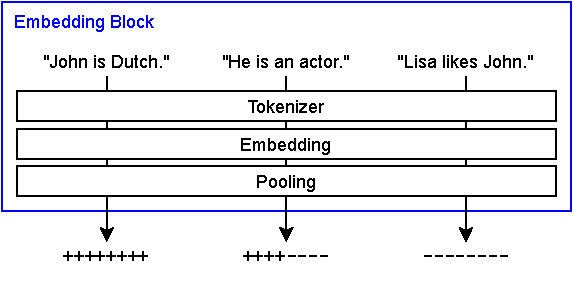
\includegraphics{4_approach/1_texter/1_text_embedding/embedding_block}
    \caption{The Texter's embedding block tokenizes sentences, embedds the tokens and combines the token embeddings to sentence embeddings in its pooling layer. Each sentence is processed individually. "+" and "-" denote positive and negative values in embedding vectors.}
    \label{fig:4_approach/1_texter/1_text_embedding/embedding_block}
\end{figure}

There are different possibilities for the concrete implementation of the individual parts, some of which will be examined in Chapter~\ref{ch:5_experiments}. In the final version of the Power model, a pre-trained transformer model is used for embedding the sentences' words, more precisely DistilBERT, a "distilled" variant of the transformer encoder BERT, reduced to the essentials~\cite{Sanh2019DistilBERTAD}. In contrast to a simple lookup table, DistilBERT is able to incorporate the context of a word into its embedding, which leads to more meaningful sentence embeddings. This choice of embedding approach also affects the tokenizer, the pooling layer, and even the input sentences: Thanks to context embedding, transformers can use special tokens that add additional information to the text. While a classical model cannot decide on the basis of the sentence "Lisa likes John." whether this sentence speaks for the class $(x, has~gender, male)$, a transformer is able to do so given the appropriately marked sentence "Lisa likes [START]John[END].". Especially for long, ambigious sentences performance can be increased significantly.

Beyond the input data, the use of a transformer also affects the tokenizer and the pooling layer. The tokenizer has to apply byte pair encoding (BPE) that is commonly used by pre-trained transformers, where sentences are not only divided into words, but words are further divided into subwords, thus keeping the vocabulary of the tokenizer small and allowing to exploit homorphisms between similar words. In addition, the tokenizer inserts the [CLS] and [SEP] introduced by BERT at the beginning and end of the sentence. That way, "Lisa likes [START]John[END]." becomes "[CLS]Lisa likes [START]John[END].[SEP]". While the [SEP] token is used to separate sentences and has no further meaning here, the embedding of the [CLS] token captures the meaning of the whole sentence and is therefore used as a sentence representation in the BERT paper~\cite{Devlin2019BERTPO}. However, the Power experiments have shown that performance can be increased if the word embeddings are also included, which is why the pooling layer of the embedding block averages all of a sentence's token embeddings, including the [CLS] embedding.
